\documentclass[a4paper,ngerman]{tui-algo-seminar}
\usepackage{graphicx}
\usepackage{algorithm2e}
\usepackage{booktabs}
\usepackage{tikz}
\usepackage{hyperref}
\usepackage{float}
\usepackage{listings}
\usepackage{totpages}  % Paket für die Gesamtseitenzahl
\setlength{\footskip}{13.0pt} % keine Ahnung ^^


\usepackage[utf8]{inputenc} % Verwenden Sie utf8 für UTF-8 Zeichencodierung

\newcommand{\inhalt}{8. Gerd Fornahl Turnier 2024}
\seminar{\inhalt}
\semester{\today}
\title{\inhalt}
\author{Erik Skopp}

\usepackage{fancyhdr}  % Für individuelle Kopf- und Fußzeilen
\nolinenumbers

% Definieren des Seitenstils
\pagestyle{fancy}
\fancyhf{}  % Vorherige Kopf- und Fußzeilen-Einstellungen löschen
%\fancyfoot[Rf]{\thepage ~von \zpageref{LastPage}}  % Gesamtseitenzahl
\begin{document}

\maketitle
\thispagestyle{plain} % Seitenzahl auf Seite 1 anzeigen
\begin{abstract}
Bericht: \inhalt.\\
Das 
\end{abstract}

\tableofcontents 
\clearpage
\section{Wichtig. Bitte lesen}

Die Tabellen und Bilder hier können nur schwer in andere CMS und Medien integriert werden. Ich bitte daher dringend darum, die Bilder und Tabellen aus der Nextcloud des Ilmenauer Schachvereins zu verwenden. Die aktuellen URLs lauten wie folgt. Bitte beachten Sie, dass sich die URLs möglicherweise geändert haben, wenn Sie diesen Artikel lesen. Die Cloud unterliegt einem ständigen Wandel.
\begin{itemize}
    \item Bilder: \url{https://cloud.ilmenauer-schachverein.de/apps/files/files/89310?dir=/Events/2024_04_Gerd_Fornahl_Gedenkturnier_8/Bilder}
    \item Tabellen: \url{https://cloud.ilmenauer-schachverein.de/apps/files/files/89358?dir=/Events/2024_04_Gerd_Fornahl_Gedenkturnier_8/Tabellen}
\end{itemize}

Ich bitte außerdem darum, die Links zu den beiden Ergebnisdiensten zu integrieren. Dies verleiht nicht nur einen professionelleren Eindruck, sondern trägt auch wesentlich zur umfassenden Darstellung des Turniers bei.

\begin{itemize}
    \item Chess-Results: \url{https://chess-results.com/tnr923015.aspx?lan=0&art=9&fed=GER&turdet=YES&flag=30&snr=3}
     \item Find Chess Game: \url{https://www.findchessgames.com/index-0134,224,1131-turniere-anzeigen.html}
\end{itemize}
\clearpage
\section{Bericht}
Gerd Fornahl, einst führender Spieler und Trainer des Ilmenauer Schachvereins, hat durch seine herausragende Kinder- und Jugendarbeit das Schachleben in Ilmenau nachhaltig geprägt. Nach seiner aktiven Zeit setzte er sein Engagement als Schiedsrichter und Trainer fort. Sein unerwarteter Tod hinterließ eine tiefe Lücke in der Schachgemeinschaft, die zu seinen Ehren das Gerd-Fornahl-Gedenkturnier ins Leben rief.

Das 8. Gerd Fornahl Turnier fand am 12. April 2024 ab 19:30 im Ernst Abbe Zentrum der Technischen Universität Ilmenau statt. Diese Veranstaltung war nur durch die engagierte Zusammenarbeit des Ilmenauer Schachvereines und des Kultur- und Kommunikationszentrums (Kukos) möglich, die gemeinsam eine ideale Plattform für das Turnier schufen.

Das Turnier begann mit spannenden Partien, die die hohe Qualität und strategische Tiefe der Teilnehmer von Anfang an zeigten. Mehlhorn Uwe eröffnete das Turnier mit einem entscheidenden Sieg über Görlach Hanna und setzte damit ein starkes Zeichen für seine Ambitionen. Markus Hartung zeigte trotz einer Niederlage gegen den späteren Turniersieger Ainur Ziganshin großes Potenzial und kämpferischen Geist.

In den folgenden Runden demonstrierte Marco Geißhirt seine Stärke durch einen wichtigen Sieg über Heitmann Erik, während Stefan Schenk mit einem beeindruckenden Sieg gegen Iresh Dudeja auf sich aufmerksam machte. Die dritte Runde bot ein packendes Unentschieden zwischen Timo Jung und Stefan Schenk, und Markus Hartung spielte sich mit einem entscheidenden Sieg gegen Georg Lehmann in den Vordergrund.

Die mittleren Runden waren von hart umkämpften Matches geprägt, darunter Erik Heitmanns Auseinandersetzung mit Timo Jung und Georg Lehmanns taktisch kluger Sieg über Erik Skopp. Die fünfte und sechste Runde brachten wichtige Siege für Torsten Michael und Markus Hartung, die beide ihre taktischen Fähigkeiten in kritischen Partien unter Beweis stellten.

Das Turnier näherte sich dem Ende, und die achte Runde war von Überraschungen geprägt, einschließlich Erik Heitmanns Sieg gegen Iresh Dudeja und Georg Lehmanns strategischem Erfolg über Marco Geißhirt. In der finalen Runde lieferten Markus Eisenbach und Simon Greul starke Leistungen, die ihre Plätze in der oberen Hälfte der Tabelle sicherten.

Zum Turnierabschluss war Ainur Ziganshin mit einer perfekten Punktzahl von 9 aus 9 der unangefochtene Champion, der das Feld dominierte und durch sein beeindruckendes Spiel überzeugte. Marco Geißhirt und Uwe Mehlhorn erreichten jeweils 7,5 Punkte und folgten ihm auf den Plätzen, wobei Geißhirt dank besserer Tiebreak-Werte den zweiten Platz einnahm. Markus Hartung und Georg Lehmann komplettierten die Top 5 mit ebenfalls starken Leistungen. Ihre Erfolge zeugen von ihrem Engagement und ihrer Leidenschaft für das Schachspiel, das sie auf und abseits des Bretts ausstrahlen.

Das Turnier war ein lebhaftes Schaufenster für das Schach, voller dramatischer Wendungen und herausragender persönlicher Leistungen, die die Faszination dieses Denksports deutlich machten und das Vermächtnis von Gerd Fornahl würdigten. \\ \\
Erik Skopp \\
Ilmenauer Schachverein

\clearpage
\section{Tabellen}
\subsection{Links zu den Tabellen}
\begin{itemize}
    \item Chess-Result: \url{https://chess-results.com/Tnr923015.aspx?lan=0&art=1}
    \item Find Chess Game: \url{https://www.findchessgames.com/index-0134,224,1131-turniere-anzeigen.html}
\end{itemize}


Alle Tabellen stehen in der Cloud unter \url{https://cloud.ilmenauer-schachverein.de/apps/files/files/89358?dir=/Events/2024_04_Gerd_Fornahl_Gedenkturnier_8/Tabellen} zur Verfügung. Bitte nutzen Sie diese für die weitere Berichterstattung. 

\subsection{Startrangliste}
\begin{table}[H]
\centering
\caption{Teilnehmerliste: Sortiert nach Spielernummer}
\begin{tabular}{ccccccccc}
\hline
\textbf{TlnNr} & \textbf{Teilnehmer} & \textbf{ELO} & \textbf{NWZ} & \textbf{Verein/Ort} & \textbf{Land} & \textbf{Geburt} & \textbf{FideKenn} \\
\hline
1 & Ziganshin,Ainur & 1881 & 2198 & Ilmenauer SV & RUS & 1998 & 34111872 \\
2 & Mehlhorn,Uwe & 2019 & 1984 & SG Blau-Weiß Sta & GER & 1961 & 4619552 \\
3 & Geißhirt,Marco & 1965 & 1998 & SG Barchfeld/Bre & GER & 1990 & 4610563 \\
4 & Schenk,Stefan & 1993 & 1909 & Ilmenauer SV & GER & 1985 & 12924059 \\
5 & Lehmann,Georg & 1797 & 1585 & ESV Lok Meininge & GER & 2002 & 34613005 \\
6 & Skopp,Erik & 1710 & 1530 & Ilmenauer SV & GER & 1998 & 16201914 \\
7 & Michael,Torsten & & 1680 & Ilmenauer SV & GER & 1967 & 12982784 \\
8 & Heitmann,Erik & 1646 & 1587 & Erfurter SK & GER & 2012 & 34608940 \\
9 & Dudeja,Iresh & 1522 & 1587 & Ilmenauer SV & IND & 1992 & 25721380 \\
10 & Hartung,Markus & & 1584 & Ilmenauer SV & GER & 1987 & 16272510 \\
11 & Görlach,Hanna & 1578 & 1167 & Ilmenauer SV & GER & 2006 & 34675604 \\
12 & Eisenbach,Markus & & 1404 & Ilmenauer SV & GER & 1984 & 34663630 \\
13 & Krasnov,Ivan & & 1027 & Ilmenauer SV & RUS & 2009 & 55610650 \\
14 & Lehmann,Norik & & 970 & Ilmenauer SV & GER & 2010 & 34697195 \\
15 & Winger,Frank & & 838 & Ilmenauer SV & GER & 1964 & 16233069 \\
16 & Jung,Timo & & & Ilmenauer SV & GER & 2005 & \\
17 & Luu,Hai Phong & & & Ilmenauer SV & VIE & 2015 & \\
18 & Peukert, Jörg & & & & GER & 1974 & \\
19 & Greul,Simon & & & Ilmenauer SV & GER & 1998 & 34677577 \\
\hline
\end{tabular}
\end{table}


\clearpage


\subsection{Abschlusstabelle}
\begin{table}[H]
\centering
\caption{Rangliste: Stand nach der 9. Runde}
\begin{tabular}{cccccccccc}
\toprule
\textbf{Rang} & \textbf{Teilnehmer} & \textbf{TWZ} & \textbf{Verein/Ort} & \textbf{Land} & \textbf{S} & \textbf{R} & \textbf{V} & \textbf{Punkte} & \textbf{Buchh} \\
\midrule
1  & Ziganshin, Ainur     & 1881 & Ilmenauer SV      & RUS & 9 & 0 & 0 & 9.0 & 44.5  \\
2  & Geißhirt, Marco      & 1965 & SG Barchfeld/Br   & GER & 7 & 1 & 1 & 7.5 & 48.5  \\
3  & Mehlhorn, Uwe        & 2019 & SG Blau-Weiß St   & GER & 7 & 1 & 1 & 7.5 & 45.5  \\
4  & Hartung, Markus      & 1584 & Ilmenauer SV      & GER & 5 & 1 & 3 & 5.5 & 52.5  \\
5  & Lehmann, Georg       & 1797 & ESV Lok Meining   & GER & 5 & 0 & 4 & 5.0 & 39.5  \\
6  & Eisenbach, Markus    & 1404 & Ilmenauer SV      & GER & 4 & 2 & 3 & 5.0 & 36.0  \\
7  & Heitmann, Erik       & 1646 & Erfurter SK       & GER & 4 & 1 & 4 & 4.5 & 46.5  \\
8  & Peukert, Jörg        &      &                   & GER & 4 & 1 & 4 & 4.5 & 32.0  \\
9  & Dudeja, Iresh        & 1522 & Ilmenauer SV      & IND & 4 & 0 & 5 & 4.0 & 49.5  \\
10 & Schenk, Stefan       & 1993 & Ilmenauer SV      & GER & 3 & 2 & 4 & 4.0 & 49.0  \\
11 & Jung, Timo           &      & Ilmenauer SV      & GER & 3 & 2 & 4 & 4.0 & 45.0  \\
12 & Michael, Torsten     & 1680 & Ilmenauer SV      & GER & 3 & 2 & 4 & 4.0 & 38.5  \\
13 & Lehmann, Norik       & 970  & Ilmenauer SV      & GER & 4 & 0 & 5 & 4.0 & 34.5  \\
14 & Greul, Simon         &      & Ilmenauer SV      & GER & 4 & 0 & 5 & 4.0 & 30.5  \\
15 & Skopp, Erik          & 1710 & Ilmenauer SV      & GER & 3 & 1 & 5 & 3.5 & 35.5  \\
16 & Görlach, Hanna       & 1578 & Ilmenauer SV      & GER & 2 & 0 & 7 & 2.0 & 35.5  \\
17 & Winger, Frank        & 838  & Ilmenauer SV      & GER & 2 & 0 & 7 & 2.0 & 34.0  \\
18 & Krasnov, Ivan        & 1027 & Ilmenauer SV      & RUS & 1 & 0 & 8 & 1.0 & 27.5  \\
19 & Luu, Hai Phong       &      & Ilmenauer SV      & VIE & 0 & 0 & 9 & 0.0 & 35.5  \\
\bottomrule
\end{tabular}
\end{table}




\section{Paarungen}
\subsection{Runde 1}
\begin{table}[H]
\centering
\caption{Paarungsliste der 1. Runde des 8. Gerd Fornahl Gedenkturniers}
\begin{tabular}{cllcl}
\toprule
\textbf{Tisch} & \textbf{Weiß} & \textbf{Schwarz} & \textbf{Ergebnis} \\
\midrule
1 & Hartung, Markus & Ziganshin, Ainur & 0 - 1 \\
2 & Mehlhorn, Uwe & Görlach, Hanna & 1 - 0 \\
3 & Eisenbach, Markus & Geißhirt, Marco & 0 - 1 \\
4 & Schenk, Stefan & Krasnov, Ivan & 1 - 0 \\
5 & Lehmann, Norik & Lehmann, Georg & 0 - 1 \\
6 & Skopp, Erik & Winger, Frank & 1 - 0 \\
7 & Jung, Timo & Michael, Torsten & ½ - ½ \\
8 & Heitmann, Erik & Luu, Hai Phong & 1 - 0 \\
9 & Peukert, Jörg & Dudeja, Iresh & 0 - 1 \\
\bottomrule
\end{tabular}
\end{table}

\subsection{Runde 2}
\begin{table}[H]
\centering
\caption{Paarungsliste der 2. Runde des 8. Gerd Fornahl Gedenkturniers}
\begin{tabular}{cllcl}
\toprule
\textbf{Tisch} & \textbf{Weiß} & \textbf{Schwarz} & \textbf{Ergebnis} \\
\midrule
1 & Ziganshin, Ainur & Skopp, Erik & 1 - 0 \\
2 & Lehmann, Georg & Mehlhorn, Uwe & 0 - 1 \\
3 & Geißhirt, Marco & Heitmann, Erik & 1 - 0 \\
4 & Dudeja, Iresh & Schenk, Stefan & 1 - 0 \\
5 & Michael, Torsten & Hartung, Markus & 0 - 1 \\
6 & Görlach, Hanna & Jung, Timo & 0 - 1 \\
7 & Winger, Frank & Eisenbach, Markus & 0 - 1 \\
8 & Krasnov, Ivan & Peukert, Jörg & 0 - 1 \\
9 & Luu, Hai Phong & Lehmann, Norik & 0 - 1 \\
\bottomrule
\end{tabular}
\end{table}

\subsection{Runde 3}
\begin{center}
\captionof{table}{Paarungsliste der 3. Runde des 8. Gerd Fornahl Gedenkturniers}
\begin{tabular}{cllcl}
\toprule
\textbf{Tisch} & \textbf{Weiß} & \textbf{Schwarz} & \textbf{Ergebnis} \\
\midrule
1 & Geißhirt, Marco & Ziganshin, Ainur & 0 - 1 \\
2 & Mehlhorn, Uwe & Dudeja, Iresh & 1 - 0 \\
3 & Jung, Timo & Schenk, Stefan & ½ - ½ \\
4 & Hartung, Markus & Lehmann, Georg & 1 - 0 \\
5 & Skopp, Erik & Eisenbach, Markus & ½ - ½ \\
6 & Heitmann, Erik & Lehmann, Norik & 1 - 0 \\
7 & Peukert, Jörg & Michael, Torsten & ½ - ½ \\
8 & Winger, Frank & Görlach, Hanna & 1 - 0 \\
9 & Luu, Hai Phong & Krasnov, Ivan & 0 - 1 \\
\bottomrule
\end{tabular}
\end{center}

\subsection{Runde 4}
\begin{center}
\captionof{table}{Paarungsliste der 4. Runde des 8. Gerd Fornahl Gedenkturniers}
\begin{tabular}{cllcl}
\toprule
\textbf{Tisch} & \textbf{Weiß} & \textbf{Schwarz} & \textbf{Ergebnis} \\
\midrule
1 & Ziganshin, Ainur & Mehlhorn, Uwe & 1 - 0 \\
2 & Dudeja, Iresh & Geißhirt, Marco & 0 - 1 \\
3 & Jung, Timo & Heitmann, Erik & 1 - 0 \\
4 & Eisenbach, Markus & Hartung, Markus & 0 - 1 \\
5 & Schenk, Stefan & Peukert, Jörg & 1 - 0 \\
6 & Lehmann, Georg & Skopp, Erik & 1 - 0 \\
7 & Michael, Torsten & Krasnov, Ivan & 1 - 0 \\
8 & Görlach, Hanna & Luu, Hai Phong & 1 - 0 \\
9 & Lehmann, Norik & Winger, Frank & 0 - 1 \\
\bottomrule
\end{tabular}
\end{center}
\clearpage
\subsection{Runde 5}
\begin{center}
\captionof{table}{Paarungsliste der 5. Runde des 8. Gerd Fornahl Gedenkturniers}
\begin{tabular}{cllcl}
\toprule
\textbf{Tisch} & \textbf{Weiß} & \textbf{Schwarz} & \textbf{Ergebnis} \\
\midrule
1 & Mehlhorn, Uwe & Ziganshin, Ainur & 0 - 1 \\
2 & Geißhirt, Marco & Jung, Timo & ½ - ½ \\
3 & Hartung, Markus & Dudeja, Iresh & 1 - 0 \\
4 & Skopp, Erik & Schenk, Stefan & 1 - 0 \\
5 & Heitmann, Erik & Michael, Torsten & 1 - 0 \\
6 & Peukert, Jörg & Lehmann, Georg & ½ - ½ \\
7 & Winger, Frank & Eisenbach, Markus & 0 - 1 \\
8 & Krasnov, Ivan & Lehmann, Norik & 1 - 0 \\
9 & Luu, Hai Phong & Görlach, Hanna & 0 - 1 \\
\bottomrule
\end{tabular}
\end{center}

\subsection{Runde 6}
\begin{center}
\captionof{table}{Paarungsliste der 6. Runde des 8. Gerd Fornahl Gedenkturniers}
\begin{tabular}{cllcl}
\toprule
\textbf{Tisch} & \textbf{Weiß} & \textbf{Schwarz} & \textbf{Ergebnis} \\
\midrule
1 & Ziganshin, Ainur & Geißhirt, Marco & ½ - ½ \\
2 & Jung, Timo & Mehlhorn, Uwe & ½ - ½ \\
3 & Dudeja, Iresh & Skopp, Erik & ½ - ½ \\
4 & Schenk, Stefan & Heitmann, Erik & 0 - 1 \\
5 & Lehmann, Georg & Winger, Frank & 1 - 0 \\
6 & Michael, Torsten & Peukert, Jörg & ½ - ½ \\
7 & Görlach, Hanna & Hartung, Markus & 0 - 1 \\
8 & Eisenbach, Markus & Krasnov, Ivan & 1 - 0 \\
9 & Lehmann, Norik & Luu, Hai Phong & 1 - 0 \\
\bottomrule
\end{tabular}
\end{center}

\subsection{Runde 7}
\begin{center}
\captionof{table}{Paarungsliste der 7. Runde des 8. Gerd Fornahl Gedenkturniers}
\begin{tabular}{cllcl}
\toprule
\textbf{Tisch} & \textbf{Weiß} & \textbf{Schwarz} & \textbf{Ergebnis} \\
\midrule
1 & Mehlhorn, Uwe & Ziganshin, Ainur & ½ - ½ \\
2 & Geißhirt, Marco & Dudeja, Iresh & ½ - ½ \\
3 & Hartung, Markus & Jung, Timo & 1 - 0 \\
4 & Skopp, Erik & Michael, Torsten & 1 - 0 \\
5 & Heitmann, Erik & Lehmann, Georg & ½ - ½ \\
6 & Peukert, Jörg & Schenk, Stefan & 0 - 1 \\
7 & Winger, Frank & Görlach, Hanna & 1 - 0 \\
8 & Krasnov, Ivan & Eisenbach, Markus & 0 - 1 \\
9 & Luu, Hai Phong & Lehmann, Norik & 0 - 1 \\
\bottomrule
\end{tabular}
\end{center}

\subsection{Runde 8}
\begin{center}
\captionof{table}{Paarungsliste der 8. Runde des 8. Gerd Fornahl Gedenkturniers}
\begin{tabular}{cllcl}
\toprule
\textbf{Tisch} & \textbf{Weiß} & \textbf{Schwarz} & \textbf{Ergebnis} \\
\midrule
1 & Ziganshin, Ainur & Dudeja, Iresh & 1 - 0 \\
2 & Jung, Timo & Geißhirt, Marco & 0 - 1 \\
3 & Eisenbach, Markus & Mehlhorn, Uwe & ½ - ½ \\
4 & Schenk, Stefan & Hartung, Markus & 1 - 0 \\
5 & Lehmann, Georg & Heitmann, Erik & 0 - 1 \\
6 & Michael, Torsten & Winger, Frank & ½ - ½ \\
7 & Görlach, Hanna & Peukert, Jörg & 0 - 1 \\
8 & Lehmann, Norik & Krasnov, Ivan & 1 - 0 \\
9 & Luu, Hai Phong & Skopp, Erik & 0 - 1 \\
\bottomrule
\end{tabular}
\end{center}

\subsection{Runde 9}
\begin{center}
\captionof{table}{Paarungsliste der 9. Runde des 8. Gerd Fornahl Gedenkturniers}
\begin{tabular}{cllcl}
\toprule
\textbf{Tisch} & \textbf{Weiß} & \textbf{Schwarz} & \textbf{Ergebnis} \\
\midrule
1 & Mehlhorn, Uwe & Ziganshin, Ainur & ½ - ½ \\
2 & Geißhirt, Marco & Hartung, Markus & 1 - 0 \\
3 & Skopp, Erik & Jung, Timo & 1 - 0 \\
4 & Heitmann, Erik & Schenk, Stefan & ½ - ½ \\
5 & Peukert, Jörg & Lehmann, Georg & 1 - 0 \\
6 & Winger, Frank & Michael, Torsten & ½ - ½ \\
7 & Krasnov, Ivan & Görlach, Hanna & 1 - 0 \\
8 & Eisenbach, Markus & Lehmann, Norik & 1 - 0 \\
9 & Luu, Hai Phong & Dudeja, Iresh & 1 - 0 \\
\bottomrule
\end{tabular}
\end{center}



\section{Bilder}
Alle Bilder stehen in der Cloud unter \url{https://cloud.ilmenauer-schachverein.de/apps/files/files/89310?dir=/Events/2024_04_Gerd_Fornahl_Gedenkturnier_8/Bilder} zur Verfügung. Bitte nutzen Sie diese für die weitere Berichterstattung.

\subsection{Siegerehrung Bild 1}
\begin{center}
    \includegraphics[width=\linewidth]{2024_04_Gerd_Fornahl_Gedenkturnier_8_01}
    \captionof{figure}{Siegerehrung Bild 1}
    \label{fig:gerd_fornahl_1}
\end{center}

\subsection{Siegerehrung Bild 2}
\begin{center}
    \includegraphics[width=\linewidth]{2024_04_Gerd_Fornahl_Gedenkturnier_8_02}
    \captionof{figure}{Siegerehrung Bild 2}
    \label{fig:gerd_fornahl_2}
\end{center}

\subsection{Siegerehrung Bild 3}
\begin{center}
    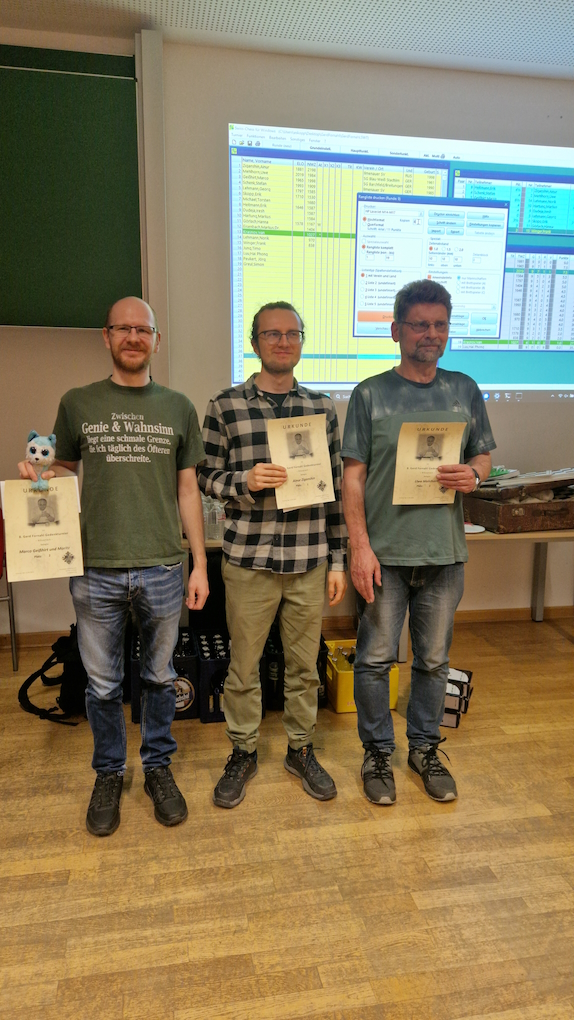
\includegraphics[width=\linewidth]{2024_04_Gerd_Fornahl_Gedenkturnier_8_03}
    \captionof{figure}{Siegerehrung Bild 3}
    \label{fig:gerd_fornahl_3}
\end{center}

\subsection{Siegerehrung Bild 4}
\begin{center}
    \includegraphics[width=\linewidth]{2024_04_Gerd_Fornahl_Gedenkturnier_8_04}
    \captionof{figure}{Siegerehrung Bild 4}
    \label{fig:gerd_fornahl_4}
\end{center}

\clearpage
\section{Anhang}
\bibliography{2024_04_Gerd_Fornahl_Gedenkturnier_8/literatur}

\end{document}
